
%% bare_conf.tex
%% V1.3
%% 2007/01/11
%% by Michael Shell
%% See:
%% http://www.michaelshell.org/
%% for current contact information.
%%
%% This is a skeleton file demonstrating the use of IEEEtran.cls
%% (requires IEEEtran.cls version 1.7 or later) with an IEEE conference paper.
%%
%% Support sites:
%% http://www.michaelshell.org/tex/ieeetran/
%% http://www.ctan.org/tex-archive/macros/latex/contrib/IEEEtran/
%% and
%% http://www.ieee.org/



\documentclass[10pt, conference, letterpaper]{IEEEtran}
\IEEEoverridecommandlockouts
\usepackage[bookmarks=false]{hyperref}
\usepackage{cite}
\usepackage[dvips]{graphicx}
\usepackage[cmex10]{amsmath}
\usepackage{caption}
\usepackage{array}
\usepackage{verbatim}
\usepackage{mdwmath}
\usepackage{mdwtab}
\usepackage{eqparbox}
\usepackage{fixltx2e}
\usepackage{stfloats}
\usepackage{url}
\usepackage{color}
\usepackage{listings}
\usepackage{makecell}
\usepackage{xcolor}
\usepackage{amsmath}
\usepackage{graphicx}
\usepackage{subfigure}
\usepackage{float}
\usepackage{booktabs}
\hyphenation{op-tical net-works semi-conduc-tor}
\usepackage{algorithm}
\usepackage{algorithmic}
\usepackage{color}
%\usepackage{algpseudocode}
\renewcommand{\algorithmicrequire}{\textbf{Input:}}
\renewcommand{\algorithmicensure}{\textbf{Output:}}



% Add the compsoc option for Computer Society conferences.
%
% If IEEEtran.cls has not been installed into the LaTeX system files,
% manually specify the path to it like:
% \documentclass[conference]{../sty/IEEEtran}





\hyphenation{op-tical net-works semi-conduc-tor}



\begin{document}

% paper title
% can use linebreaks \\ within to get better formatting as desired
\title{MicroPrivacy: \\Detection of Visual Eavesdroppers on Smartphones}
%Detection of Visual Eavesdroppers to Preserve Privacy on Smartphones }


% author names and affiliations
% use a multiple column layout for up to three different
% affiliations

%\author{
%\IEEEauthorblockN{Hui Wen$^{1,2}$, Qiang Li$^{1,2}$, Qi Han$^{3}$, Shiming Ge$^{1}$,Limin Sun$^{1}$\thanks{\small{Limin Sun is the corresponding author.}}
%}
%\IEEEauthorblockA{
%$^1$Institute of Information Engineering,CAS,Beijing, Beijing, China 100093
%\\$^2$University of Chinese Academy of Sciences, Beijing, China 100093
%\\$^3$Department of EECS, Colorado School of Mines, Golden, CO USA 80401
%\\ Email:\{{wenhui,liqiang43,geshiming,sunlimin\}}@iie.ac.cn, qhan@mines.edu
%}
%
%}

\author{}


% make the title area
\maketitle


%\begin{abstract}
%%\boldmath
%Visual eavesdropping refers to a scenario that a person tries to read the content displayed on another person's mobile phone screen over the shoulder of that person while trying to be unobtrusive.
%We present an interesting approach that detects visual eavesdroppers in order to preserve privacy on mobile phones. The proposed detection method relies on computer vision and image processing algorithms running on the video streams from the front camera  built in most commodity mobile phones.
%Considering the limitations of a mobile phone's computation power and camera's field of view, we propose effective pre-processing techniques to reduce computation needs.  We further combine face detection and motion detection methods to improve the accuracy for detecting  visual eavesdroppers in different scenes. For situations in which a visual eavesdropper moves into an area not detectable by the front camera, we design a maximum likelihood estimation method to predict the probability of potential visual eavesdropping.
%We present the design and implementation of visual eavesdroppers detection method.  We evaluate the proposed method using a series of experiments.  Our empirical studies show that the proposed technique achieves high detection accuracy.
%\end{abstract}

\begin{abstract}

In this paper, we define a `micro-privacy in macro-place' privacy violation issue and proposed a computer vision (CV) based method to address this problem. Specifically, when a user is using his phone, another person close to him tries to read from his phone screen.  We refer to this person as `a visual eavesdropper.'  Our idea is to use the front camera of smartphone as the eye on the back to preserve phone screen privacy  in the public place.  We present {\it MicroPrivacy},  the first computer vision based system that integrates image and video processing techniques on smartphones to effectively detect visual eavesdropping.  MicroPrivacy deals with the limited camera view issue and the constrained computation power of smartphones.
%We divide the privacy area into two parts: area inside the front camera view and area outside of the front camera view. Within the camera view area, we adopt vision and image processing algorithms to detect visual eavesdroppers; outside the area, we predict the location of the eavesdropper based on his previous direction and speed.
We validate the effectiveness of MicroPrivacy on CV public data and private data that we collected from real world. Experimental results on the datasets demonstrate that MicroPrivacy achieves  proper precision and recall in detection of visual eavesdroppers.

%MicroPrivacy performance is acceptable and practical for preserving people micro-privacy on smartphone screen.
\end{abstract}

\begin{IEEEkeywords}
Smartphone privacy; Mobile applications; Face detection
\end{IEEEkeywords}



\IEEEpeerreviewmaketitle



\section{Introduction}
% no \IEEEPARstart

% the importance of the privacy
% privacy protection method
% background
% intuitive method
% details

%importance of visual privacy
As the usage of smartphone becomes part of our daily lives and our public surroundings are increasing, people are more eager than ever to create their own personal space using the small and micro-private smartphone screen.  However, light-emitting phone screens are naturally attention grabbing, easily seen by  people around, so they can easily become the target of privacy violation.
For instance,  on a subway train,  Alice is reading an instant message from her intimate friend, people behind her maybe eavesdrop the screen leading to leakage of the private information. Alice might feel uncomfortable about it whether eavesdropper is innocuous or hostile.


In this paper, we address this micro-privacy issue with  smartphone screen in a public space, e.g., subway station, train, bus, office, cafe,  classroom, or plaza.  We consider  the person who watches another person's smartphone screen without the user's awareness as a visual eavesdropper and define this behavior as  visual eavesdropping.
We found that it is a new  privacy issue only proposed recently and in urgent need of  a protection  or warning strategy to help a phone user to avoid being visually eavesdropped.  Hand-shielding gesture is used to prevent password from being seen by others\cite{yan2013designing}, but it is obtrusive and it is hard to require a user to protect his screen all the time while he is busy texting or browsing. There, we aim to design an automatic method to solve this privacy problem.
\begin{figure}[!htb]
\centering
\includegraphics[width=3.5in]{first.eps}
\caption{An example of visual eavesdropping}
\label{fig:motivation}
\end{figure}

To avoid visual eavesdropping, it is better not to rely on any other additional device other than the user's phone being used. 
Most modern commodity smartphones  have embedded a front camera, we propose to use that to serve as the eye at the user's back and then use a computer vision (CV) based method for detection of visual eavesdropping. 



While the idea of using the CV(Computer Vison) based method with the front camera to detect visual eavesdropping seems straightforward, many interesting challenges arise in practice.
First,  the camera field of view is limited.
Evidently, the necessary prerequisite of detection is that a visual eavesdropper should be captured by the front camera. However, due to the limited camera view, a visual eavesdropper might fall outside of the camera view but still can read the phone screen.
Also, a user may read his messages on his phone while walking. The front camera  can hardly see the object clearly because of the motion blur.
Second,  the phone user's face always blocks the camera view.  This blocking essentially exacerbates the limited camera view  problem.
Last, a fast real-time visual detection algorithm typically requires lots of computation resources that a smartphone may not afford to, so it is hard to achieve both high detection accuracy and speed in visual detection.

 % our approaches
In this paper, we  these challenges as follows. % detection of visual eavesdroppers on smartphones.
To address the problem of limited field view of front camera, we divide the privacy area into two parts: the area inside the camera view and the area outside of the camera view. For the area inside, we propose a visual detection algorithm to identify visual eavesdroppers; for the area outside, we pre-estimate the movement speed and direction of the visual eavesdropper while he is inside the area, and then predict the probability of the area that  visual eavesdroppers may appear.
To address the problem of  the phone user blocking camera, we replace the area blocked with a consistent background. We calculate the size of the blocked area to predict the probability of the visual eavesdropper may appear in this area.
To address the problem of motion blur caused by moving, we adapt the motion deblur technique \cite{deblur}. To address the limited computation capabilities of smartphones, we include a strategy that removes the blocked area before visual detection.

%We address these challenges using several strategies. Firstly, we determine the size of the privacy impaired area where a visual eavesdropper may potentially exist.  {\color{red} modify! There is a tradeoff in the size of the privacy impaired area. } If  it is too small, we will miss some areas with potential eavesdropping; if it is too large, the computation cost is too high to afford.  Therefore,  defining a proper privacy impaired area not only improves detection accuracy and speed, but also reduces unnecessary energy consumption on phones. {\color{red} delete! Secondly, when we use the images captured by the front camera to detect visual eavesdroppers, we  remove the area blocked by user's face. }  This can reduce computation cost. Thirdly, we propose a robust detection method that considers different situations such as when a visual eavesdropper is outside the camera's view or when the background is complex. {\color{red} need to use a different word than complex. }
%Finally, we take into account dynamics in environments to fine tune our approach to be adaptive.  For instance,  how long a person watches your phone is considered visual eavesdropping has a lot to do with environmental factors.

%In this paper, we propose an visual eavesdroppers detection method for protecting the visual privacy. In stead of developing new human detection algorithms, we integrate the face detection and body detection to improve the robustness of the visual human detection. We further proposed an invisible human prediction model to calculate the probability of the person who is peeping at your phone in the area that falls out of the camera monitoring area.

%We validate the effectiveness of  MicroPrivacy using public datasets and also the data we collected from real world over three months.


In brief, we have made the following contributions in this work.
\begin{itemize}
\item We present a visual privacy issue on the smartphone screen that easily leaks out private information.  
\item We propose a new method to use the front camera of a smartphone to act as a human eye at the back.
\item We implement MicroPrivacy, the first computer vision based system to detect visual eavesdroppers under the constraints of limited camera view and computational power of smartphones.
We integrated several CV based techniques  for handling different situation in real world.
\item We evaluate MicroPrivacy  using both public datasets. Experimental results show that MicroPrivacy  achieves high precision and recall in detecting visual eavesdroppers. It also requires 20\% less computational power while still guaranteeing the same detection accuracy.
\item We conduct real world experiments and results show that MicroPrivacy is practical for preserving people micro-privacy on smartphone screen.
\end{itemize}

The rest of the paper is structured as follows.
We present  related work about privacy in Section II and show the difference between them and our approach.
We describe the system design considerations of MicroPrivacy  in  Section III.
We then present details of MicroPrivacy, including three parts: privacy definition, visible human detection and invisible human detection in Section IV.
In Section V,  we report our  experimental results.
Finally, we make final remarks and discuss the limitations of our approach in Sections VI. 




\section{Related Work}


Privacy is recognized as a dominant concerning factor for a mobile device, in particular for smartphones.
Several pieces of work have studied how to protect user privacy by detecting  behaviors   accessing sensitive data.
TapPrints~\cite{tapprints2012} uses motion sensors (i.e, accelerometer and gyroscope) to infer the location of taps on the touch screens and detect smartphone-sensitive data such as password.
TaintDroid~\cite{taintdroid2014} provides an Android's virtualized execution environment to analyze and determine whether third-party applications leak out user  privacy data or not.
Similarly,  PiOS~\cite{pios2011} conducts a static analysis over iOS application intermediate code to discover any possible leaks of sensitive information by third parties. EnCore~\cite{encore2014} introduces a privacy preserving approach for mobile social applications, where people encounter strangers within a wide range of communication.
In contrast, our work focuses on a totally different privacy on smartphones, micro-privacy on screen.
A light-emitting phone screen maybe leak  out phone user's privacy information in the public area.

To protect user privacy, it is important to distinguish from a malicious behavior.
RiskRanker~\cite{riskranker2012} identifies and assesses potential security risks from  untrusted apps to defend against malware.
MAdFraud~\cite{madfraud2014} studies advertisement fraud issues that is displayed on app's GUI and is embedded with Ad libraries from  the ad provider on mobile phones.
Differently, our work proposes to preserve user privacy via issuing an alert/alarm to users, where the front camera acts as an eye on the back.
The front camera identifies the scene that a phone user's private information might be leaking out.


Similar to our work, several smartphone applications also adopt the front camera for different purposes. 
Carsafe~\cite{carsafe2013} protects a  driver safety by alerting drivers to dangerous driving conditions and behavior. It uses  the front camera to monitor the driver  status and the rear camera to detect road conditions.
Our work also uses the front camera, but we use it to detect visual eavesdroppers to protect user privacy.
ViRi~\cite{viri2013} restores the front-view effect at the  slanted viewing angle to help users  see smartphone screen content conveniently. It uses the front camera  to  determine whether the screen is needed to slant a certain angle and adds  a commercial off-the-shelf fisheye lens to address  the limited field view of the front camera.
Our work comes from a different perspective. it is common that people  carry and use their phones when they are in public areas. It is impractical and inconvenient to require a user to pre-setup a fisheye lens  on the front camera to detect visual eavesdroppers. Therefore, our approach does not depend on the addition of an extra hardware. 

\input{design_Consideration.tex}

\section{System Detailed Design}
\label{sec:details}

In this section, we first present the overview of MicroPrivacy, then describe the details of each key component.

Figure~\ref{fig:architecture} shows the proposed MicroPrivacy framework.
In  Layer 1,  six modules are used: smartphone tilt angle, camera view angle, and angle of potential eavesdroppers, motion detection, face detection, and body detection.
We assume that three types of sensors are embedded into smartphones to act as input data for Layer 1, i.e, accelerator and gyroscope are used to estimate smartphone tilt angle, and camera sensor is used to capture image frames.
These modules provide input data for Layer 2.
In Layer 2, there are three key components:  (1) \textit{Privacy area Estimation} determines the area where potential visual eavesdropping may occur. (2) \textit{Visual detection inside the camera view} combines face detection and motion detection  to detect human visible by the camera. (3) \textit{Prediction outside the camera view} predicts the probability of visual eavesdroppers based on the estimated movement speed and direction of the eavesdropper while he's inside the camera monitoring area.
In Layer 3,  the visual eavesdropper detection algorithm determines whether to alert the user or not.

\begin{figure}[H]\label{framework}
\centering
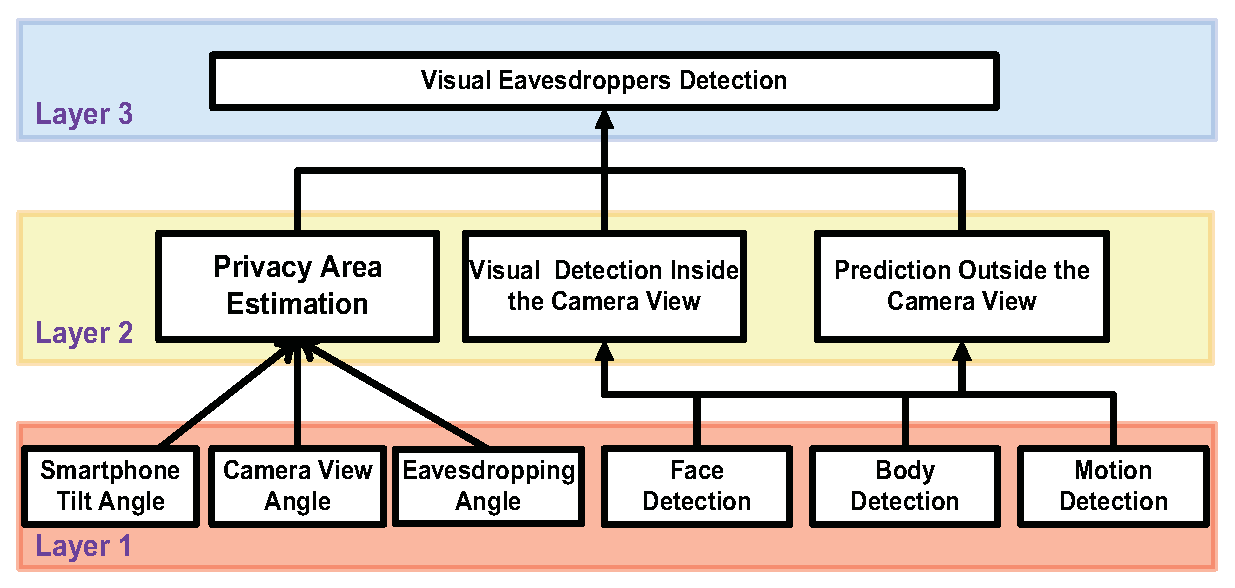
\includegraphics[width=3.5in]{framework.eps}
\caption{Architecture of  visual eavesdroppers detection}
\label{fig:architecture}
\end{figure}

\subsection{Privacy Area Estimation}

The size of the privacy area determines the scope the front camera is able  to cover.
First, we  define four types of areas to represent the situation that the visual eavesdropper detection algorithm works differently.
We then derive a formula to estimate the size of the privacy area taking into account  the visual distance, and the phone tilt angle, and the area blocked by user.

\subsubsection{Definition of the Privacy Area}
As Fig.~\ref{fig:area} shows, the red area (i.e., the monitoring area) represents the front camera field of view and the blue area (i.e., the privacy impaired area) shows the range that the visual eavesdroppers can see the information on smartphone screen. The overlap of the two areas is denoted as $A_{11}$, the part of the impaired area that is out of the monitoring area is denoted as  $A_{10}$,  the part of the monitoring area that falls out of the privacy impaired area is denoted as $A_{01}$,  and the area that is outside both monitoring and privacy impaired areas is $A_{00}$. Typically, $A_{01}$ is  very small  and $A_{00}$ is the unconcerned area. We further use $\alpha_h$, $\alpha_v$ to represent the horizontal and vertical angle of the camera view respectively. The angle of potential eavesdropping is defined as $\beta$. Therefore, at  distance $d$, the monitoring area  (i.e., $(A_{11}+A_{01})_d$) can be expressed as $d^2\tan^2\beta$ and the privacy impaired area  (i.e., $(A_{11}+A_{10})_d$) is $d^2\tan\alpha_v\tan\alpha_h$.
\begin{figure}[H]
\centering
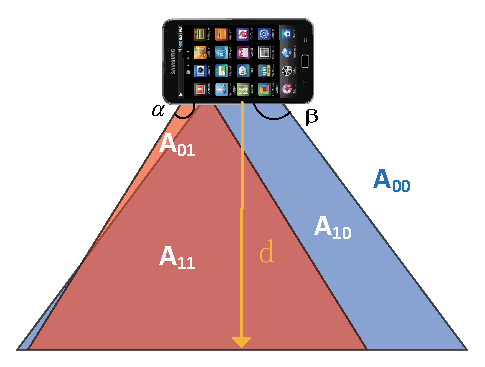
\includegraphics[width=2in]{area1.eps}
\caption{Definition of different areas }
\label{fig:area}
\end{figure}


\subsubsection{Issues for Determining Area Size}


The size of privacy impaired area is affected by three factors:  visual distance $d$,  phone  tilt angle $\theta$, and size of the area blocked by user.

\textbf{Visual distance.} To estimate the privacy area, we should measure the maximum visual distance that a person can see the text on smartphone (Fig.~\ref{fig:distance}). In our daily life, we use the eye chart to measure the visual acuity (i.e., how far  a person can see clearly). We determine the visual distance by considering the phone screen as an eye chart with the international definition of visual acuity \cite{acuity}.  The visual distance is expressed as:
\begin{equation}
\begin{split}
& d=\frac{acuity*font size}{gap size*tan\theta^*}
\end{split}
\end{equation}
where $\theta^*=0.0167$ is a visual angle of 5 arc minutes and $gapsize$ is 5 based on the design of a typical optotype. \textit{Acuity} is the value used in the international definition of visual acuity and we set acuity value to 20/20=1.0, the standard visual range of the human.  \textit{fontsize} represents the height of the font on the phone screen. The screen size of the smartphone  ranges from 3 inches to 6 inches and font size is no larger than 10.7 mm. This gives the maximum visual distance of 5 meters.
\begin{figure}[H]
\centering
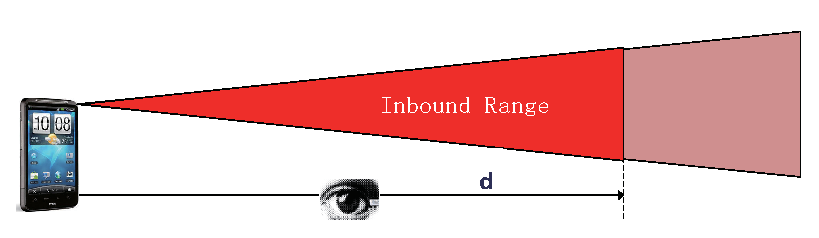
\includegraphics[width=3.5in]{distance.eps}
\caption{Estimation of  visual distance}
\label{fig:distance}
\end{figure}


\textbf{Tilt angle of the phone.}
The phone rotation affects the area size (Fig.~\ref{fig:rotation}).  With the angle of the phone rotation $\theta$ and distance $d$, the monitoring area is  $d^2\tan^2\beta\tan\theta$ and  privacy impaired area is $d^2\tan\alpha_w\tan\alpha_h\tan\theta$.
\begin{figure}[H]
\centering
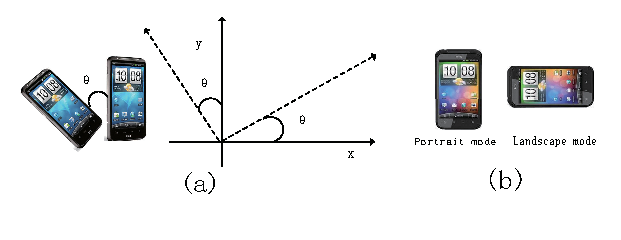
\includegraphics[width=3.5in]{rotation.eps}
\caption{(a) The angle of the phone rotation (b) The camera view mode}
\label{fig:rotation}
\end{figure}

\textbf{Size of user-blocked area.}
When the camera view of the smartphone is blocked by the user's face, the blocked area has no use for face detection and affect the performance of the visual eavesdroppers, even though it is part of the monitoring area, so we need to determine the size of the blocked area (Fig.~\ref{fig:block}).
\begin{figure}[H]
\centering
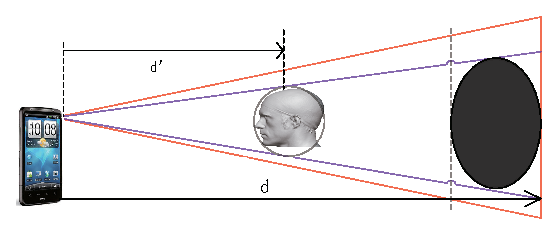
\includegraphics[width=3.5in]{blockedarea.eps}
\caption{The user's face blocks the camera view }
\label{fig:block}
\end{figure}

Assume that the face height in the camera is defined as $f_h$ and the camera focus is expressed as $fos$ (available through Android API), we can derive the distance $d'$ between face and camera by using the pinhole camera model \cite{PinholeModel}. The pinhole camera model describes the mathematical relationship between the coordinates of a point and its projection onto the image plane of an ideal pinhole camera.
\begin{equation}
d'=\frac{fos*face\_height}{f_h}
\label{eqn:d'}
\end{equation}
where $face\_height$ is the actual face height in millimeters,
$f_h=\frac{f_h(p)*res_h}{s_h*dpi*0.3937}$, note that 1 cm $\approx$ 0.3937  inches.  $f_h(p)$ is the face height measured in pixels on smartphone, dpi is dots per inch, $res_h$ is screen height resolution  and  $s_h$ is image height size.  They can all be obtained via Android APIs.
%The face height $f_h$ can be calculated by the face height . Android APs can provide the dpi (dots per inch), screen height resolution $res_h$ and image height size $s_h$, so we can compute face height in camera $f_h=\frac{f_h(p)*res_h}{s_h*dpi*0.3937}$  (1 cm $\approx$ 0.3937  inches.).
The range of the face size is limited and the  estimation of the face size is difficult. Therefore, we set the face height to the average size of 220mm instead of estimating one's actual face height. Therefore, we can use Eq.~\ref{eqn:d'} to calculate the distance $d'$ between camera and face. %For estimating the blocked area at distance $d$, we need to know the face height $f_h$ and width $f_w$ in camera.
The aspect ratio of face width and height in an image is the same as in reality, so with the face width measured in pixels available via Android API, we can compute $f_w$ in a similar way as computing $f_h$.  Therefore,
\begin{equation}
\textrm{size of blocked area} = f_w*f_h\frac{d}{d'}
\end{equation}


\subsubsection{Computation of Privacy Area Size }
To calculate size of the monitoring and privacy impaired area, we use the tilt angle of the phone ($\theta$), camera view angle ($\alpha_v$ and $\alpha_h$), and the  angle of a potential visual eavesdropper ($\beta$). In addition, we take into account the area blocked by the phone user, which is determined by  face height ($f_h$), face width ($f_w$), and distance ($d'$).
Based on the discussions previously, we have the  size of the monitoring area and privacy impaired area at distance $d$ as follows.
\begin{equation}
\begin{split}
& (A_{11}+A_{01})_d=d^2\tan^2\beta\tan\theta-f_w*f_h\frac{d}{d'}\\ %\textrm{size of monitoring area} =
& (A_{11}+A_{10})_d=d^2\tan\alpha_w\tan\alpha_h\tan\theta-f_w*f_h\frac{d}{d'} %\textrm{size of privacy impaired area} =
\end{split}
\end{equation}


\subsection{Detection inside the camera view}
When an eavesdropper stays inside the camera view, we use a visual detection algorithm to discover him.
Given two image frames, visual human detection  aims to detect human in the monitoring area by combining face detection and body detection.

%\subsubsection{Face Detection}
Face detection can help detect human and plays a important role in detecting the visual eavesdropper. Many face detection methods have been proposed \cite{viola2004robust} and shown their effective using public datasets. The face detection APIs or libraries are available from opencv\cite{opencvFace}, android\cite{androidFaceAPI}, and other open source projects\cite{MicrosoftFace}. In MicroPrivacy, we integrate different APIs to run our system on different platforms. The basic face detection algorithm is based on the Haar cascade algorithm \cite{viola2004robust}.

%\subsubsection{Body Detection} \label{dt:motion}
Many computer vision algorithms have been designed to track and detect objects such as human body\cite{felzenszwalb2008discriminatively}\cite{wang2009hog}.  However, we adopt a motion detection method to track the body. Even with limited  computation power of mobile phones, motion detection  is still fast and effective for  camera-based apps. As Fig.~\ref{fig:motion} shows, the proposed method uses two frames to get the object and considers the center of the object as the key point for tracking.  Specifically, we use frame difference method \cite{lee2009vision} that subtracts two frame for detecting the moving object. The centroid of the moving object is considered as a key point.  %Compared with using two key points from three frames, we can easily get the motion direction and  speed. Further,
 Motion detection  can generate human trajectories  that can be very handy for potential eavesdropping even when the person is invisible in the camera.
\begin{figure}[H]
\centering
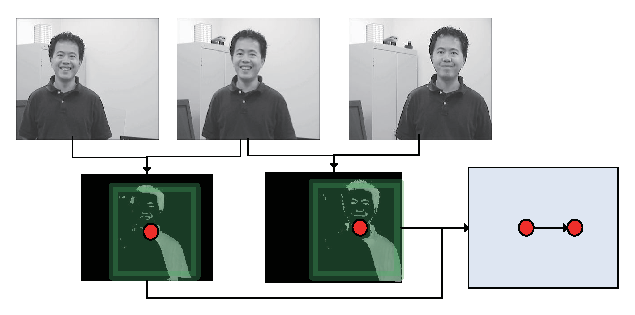
\includegraphics[width=3.5in]{motion.eps}
\caption{Motion detection using the Mhyang tracking database}
\label{fig:motion}
\end{figure}


%\subsubsection{Fast detection}
 We propose to speed up the visual detection algorithm.  Intuitively, we reduce the size of privacy area which reduces the computation of visual detection algorithm. We first remove the user-blocked area from the monitoring area of the front camera.
Usually, the smartphone user face takes a large space in the image size. Removing it will speed up  visual detection algorithm.
We then process the frames with the face-blocked area removed. In this way,  face detection can be significantly accelerated. Fig.~\ref{fig:remove} is an example of this process using the Caltech dataset~\cite{jesorsky2001robust}.
The left is the original image that consumes more computation than the right  with the face removed from the image.
\begin{figure}[H]
\centering
\includegraphics[width=3.5in]{face.eps}
\caption{Remove the blocked area for fast face detection (the original image is from the Caltech dataset)}
\label{fig:remove}
\end{figure}

%Remove the blocked area for fast face detection every few seconds from the monitoring area, we only need to detect faces in the other part.   the Face detection method can be speed up by removing the blocked area caused by the occlusion of the phone user's face. If we remove the blocked area from the monitoring area, we only need to detect faces in the other part.  %We propose a polling mechanism to implement this method. This polling mechanism locate the position of the user's face and remove it every time, just as a timer.  Specifically, We use face detection to detect the full image and remove the largest face area every few seconds. During this interval,




\subsection{Prediction outside the camera view}
A visual eavesdropper may move out of the camera's monitoring area but can still see  the phone's screen.
% if the viewer is initially in that area, then this approach will not work.
To detect this,  we estimate the probability of this situation. The basic idea  is to use the historical human trajectory to predict its next  location. If the predicted location is still in the privacy impaired area, the invisible eavesdropper is considered to be detected.

We use maximum likelihood estimation to build a probability model for this detection:
\begin{equation}
\begin{split}
& P(t,\tau|M)=P(t|M)P(\tau|M),
\end{split}
\end{equation}
where $t$ is the duration of the detected face that disappears from the monitoring area and $\tau$ is the duration of the detected  body that disappears from the monitoring area. $M$ is the parameter to be be estimated for maximizing the likelihood probability $P(M|t,\tau)$. Three aspects of the parameter $M$ can be used for determining the data distribution and they are direction, speed, and area size. %and expressed as $M=\{direction,speed,area size\}$.
We use these three elements to build a probability model to determine $M$.  Instead of obtaining $M$ from training data as a typical maximum likelihood estimation method, we get it from the human detection model;  the goal is the same, i.e., to maximize the likelihood probability $P(M|t,\tau)$.  Specifically, we use face detection and motion detection  to record the human's trajectory. Once the detected human  disappears from the camera view, we calculate the motion direction and speed from the records, predict the possible location of the human. We use the area size  to estimate the possible time duration that the invisible person can still  read the phone screen. The probability of the invisible person eavesdropping is expressed as follows (Fig.~\ref{fig:invisible}).
\begin{equation}
P(t|M)=P(\tau|M)=1-\frac{v*t}{d^*\cos\gamma(\tan\beta-\tan\alpha)+\epsilon}
\label{eqn:prob}
\end{equation}
where $v$ is the motion speed, $\gamma$ is the motion direction,  $d^*$ is the distance between object's face and camera, and  $\epsilon$ is a smoothing factor to avoid the exception of division by zero. $\alpha$ is set to $\alpha_v$ or $\alpha_h$ while the phone is in vertical ro horizontal.
%that is mentioned in \textit{Area Estimation} section.
\begin{figure}[H]
\centering
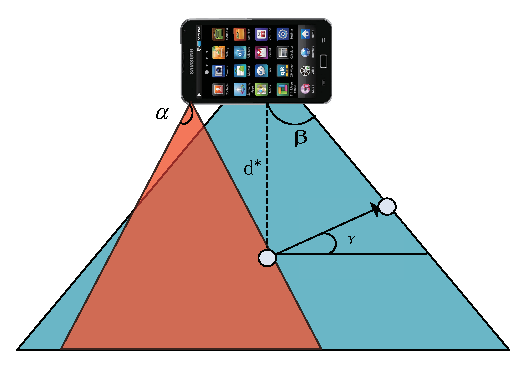
\includegraphics[width=2.5in]{areaMotion.eps}
\caption{Prediction of eavesdropper outside camera view}
\label{fig:invisible}
\end{figure}



There is another situation for predicting the location of the visual eavesdropper, i.e., the visual eavesdropper  moves into the user blocked area. This area is inside the monitoring view but is blocked by phone user's face (Fig.~\ref{fig:invisible-blocked}).
\begin{figure}[H]
\centering
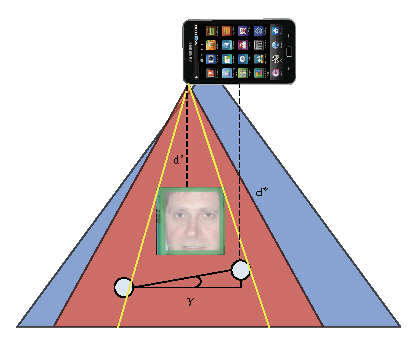
\includegraphics[width=2.5in]{areaMotionBlocked.eps}
\caption{ Human prediction in area blocked by user face}
\label{fig:invisible-blocked}
\end{figure}
In this case, the probability of the invisible human eavesdropping is expressed as:
\begin{equation}
P(t|M)=P(\tau|M)=1-\frac{v*t}{d^*\cos\gamma*(f_w*\frac{d^*}{d'})+\epsilon}
\label{eqn:prob}
\end{equation}


%The method discussed previously uses
%The two thresholds $t$ and $\tau$ used in the method discussed previously should be adaptive to the environment in terms of noise level, crowded or not, or whether many people are passing by, etc.  We propose a methodology for threshold selection (Fig.~\ref{fig:env}).   It consists of three steps.  (1) \textit{Multi-sensor Fusion} collect data from WiFi, GPS, and acoustic sensor to generate fused data.(2) \textit{Environment Perception} uses support vector machine  to classify the environment. (3) \textit{Threshold Learning} uses AdaBoost~\cite{} to learn the proper thresholds.
%\begin{figure}[H]
%\centering
%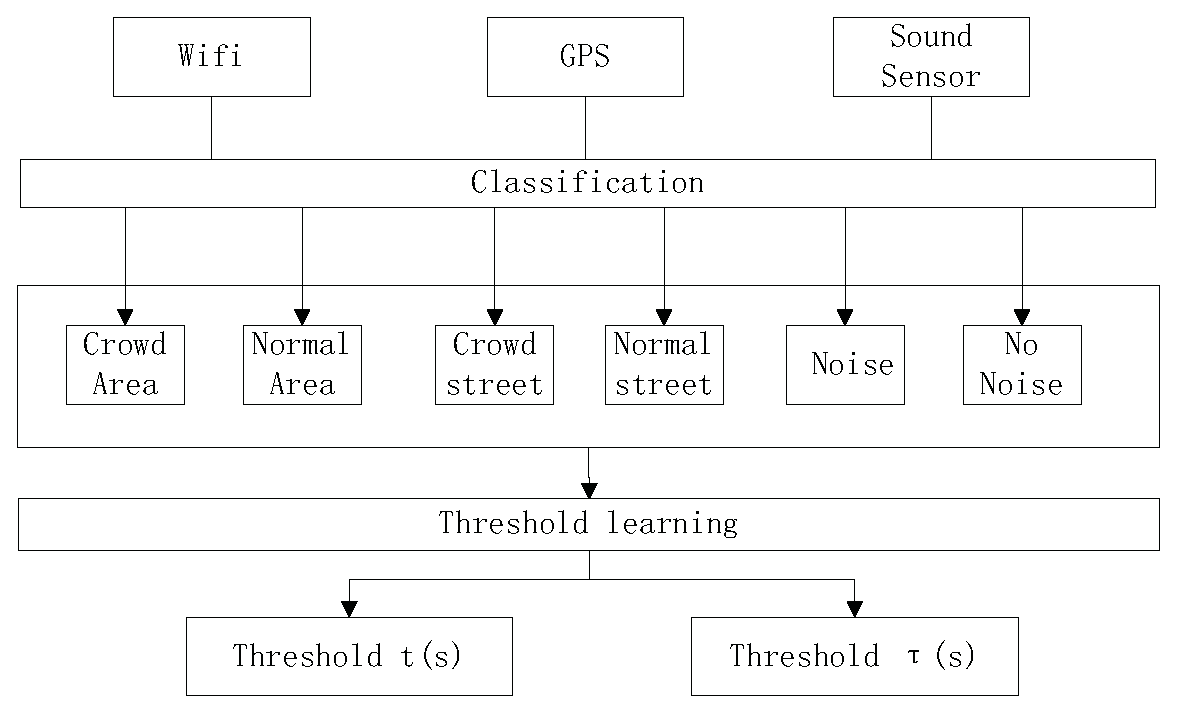
\includegraphics[width=3.5in]{sensorfusion.eps}
%\caption{The architecture of environment perception with sensor fusion.  }
%\label{fig:env}
%\end{figure}

\subsection{Visual Eavesdropper Detection Algorithm}
A visual eavesdropper is a person who stays around the user and watches the user's phone screen for a time duration longer than the threshold.  Since  we use face detection and motion detection to detect human, it is necessary to record the face detection time $t_h$ and the motion detection time $\tau_f$. If we denote   $f(\tau_f,\textit{t}_h)$ as the visual eavesdropper detection result, then
\begin{equation}
f(\tau_f,\textit{t}_h)=
\begin{cases}
1 & \text{if}\,\tau_f>\tau(s) \textrm{ or } \textit{t}_h>\textit{t}(s)\\
0 & \text{otherwise}
\end{cases}
\end{equation}
where $t_h$ represents the time of the human body in the privacy impaired area,  $\tau_f$ represents the time that the person looks at the phone screen, $\tau(s)$ and $t(s)$ are the thresholds to indicate time duration that a normal person stays.
A person is considered as a visual eavesdropper if detected face time $\tau_f$ is larger than the threshold $\tau(s)$ or detected body time $\textit{t}_h$  is larger than the threshold \textit{t}(s).
The threshold is sensitive to the environments around the smartphone user. For instance, the time threshold on the bus station should be different from the classroom.  According to the experience or the feedbacks of smartphone users, we set the time threshold $\tau(s)$ and \textit{t}(s) to empirical values.



%Putting it all together, the entire algorithm is shown in Algorithm~\ref{alg:Framework}.
Algorithm~\ref{alg:Framework} describes the overall algorithm of our visual eavesdropper detection.
We first calculate the privacy area using Eq. (4) based on camera angles ($\alpha_v,\alpha_h$), title angle of the phone ($\theta$), and visual distance ($d$) (Line~\ref{alg:line:1}).  If the front camera detectes the face of a visual eavesdropper, we add one to the time variable $\tau_f$ that represents the storage time of face detection (Line~\ref{alg:line:2}).  If the body of the eavesdropper is detected by front camera, the time variable $\tau_h$ needs to increment by one, which denotes the storage time of body detection  (Line~\ref{alg:line:3}).
%We directly added the unit time to the time variable, if  eavesdroppers are fall within the side of camera coverage.
When an eavesdropper falls outside the camera view, we use Eq.(~\ref{eqn:prob}) to calculate the time  variables $\tau_h$ and  $\tau_f$ (Line~\ref{alg:line:4})..
Finally our algorithm determines whether there is a   visual eavesdropper or not (Line~\ref{alg:line:5}).

\begin{algorithm}[H]
\caption{Visual Eavesdroppers Detection}
\label{alg:Framework}
\begin{algorithmic}[1]
\REQUIRE  face detection $t(s)$, body detection  threshold $\tau(s)$ , camera angles ($\alpha_v,\alpha_h$), title angle of the phone ($\theta$), visual distance ($d$)
\ENSURE   Visual eavesdropper detection result;
             alerts to user;
\STATE Calculate privacy area using Eq.(4);
\label{alg:line:1}
\STATE Connect to the front camera initially;
\STATE Initialize  face detection time $\tau_f=0$;
\STATE Initialize body detection time $\textit{t}_h=0$;
\REPEAT
\STATE Get the current frame from the front camera;
%\STATE Processing the received frame;
\STATE Run face detection algorithm;
\STATE Run human motion detection algorithm;
\IF  {\textit{detected  human in previous frame} }
\STATE Calculate motion direction $\gamma$ and motion speed $v$
\ENDIF
\IF  {\textit{detected  human face}}
\STATE $\tau_f=\tau_f+1$; Calculate  total face detection time
\label{alg:line:2}
\ENDIF

\IF  {\textit{tracked  motion of  human body}}
\STATE $\textit{t}_h=\textit{t}_h+1$;  Calculate  total motion detection time
\label{alg:line:3}
\ENDIF
\IF  {\textit{face detection failed} and \textit{motion detection failed}}
\STATE Estimate $R_h$ and $R_f$ based on Eq.~\ref{eqn:prob}:
\STATE $\textit{t}_h=\textit{t}_h+P(t|M)$;
\STATE $\tau_f=\tau_f+P(t|M)$;
\label{alg:line:4}
\ENDIF
\IF  {\textit{$t_h$}$\geq$\textit{t}(s) or  $\tau_f \geq\tau(s)$ }
\label{alg:line:5}
\STATE Label the human as a visual eavesdropper;
\STATE $f(\tau_f,\textit{t}_h)=1$;
\STATE $\tau_f=0$ and $\textit{t}_h=0$;
\STATE Alert the user about the  privacy leakage;
\ENDIF
\UNTIL User terminates the application




\end{algorithmic}
\end{algorithm}




\section{Performance Evaluation}


In this section, we present the performance evaluation of our proposed approach.
We first evaluate privacy area estimation  using real world measurement data.
For detection of eavesdroppers in the front camera view, we use publicly available datasets to evaluate the accuracy and speed of our face detection and motion detection.
For prediction of eavesdroppers outside the camera view, we have conducted controlled experiments to evaluate the accuracy of our prediction.
Finally, we run a prototype system in a real-world setting to evaluate the effectiveness of our overall approach to visual eavesdropping detection.

\subsection{Experiments on Privacy Area Estimation}
To evaluate our ideas on privacy area estimation, we tie a smartphone to a tablet stand so that we can keep the phone in vertical and horizontal positions on the desk as shown in Fig.~\ref{fig:area-exp}.  The phone faces a wide wall at distance $d^*$.  We use the front camera of the phone to capture images of the wall in order to get the monitoring area, and we use tape to measure the actual size of monitoring area. In this way, we can calculate the camera angle of  different smartphones in both vertical and horizontal positions at distance $d^*$.  We  then derive  the error of our distance estimation that deviates from the actual distance and the error of our size area estimation that deviates from the actual area size.
\begin{figure}[!htb]
\centering
\includegraphics[width=3.5in]{epsarea.eps}
\caption{Experimental setup for evaluation of area estimation}
\label{fig:area-exp}
\end{figure}

In these experiments,  $d^*= 2.4$m.  $R_h$ and $R_v$  are the horizontal length  of the monitoring area  measured on the wall when the smartphone is put on the desk in horizontal and vertical positions respectively.
The view angle of the camera in horizontal is $\alpha_h = arctan(\frac{d^*}{2*R_h})$ and the view angle of the camera in vertical $\alpha_v = \arctan(\frac{d^*}{2*R_v})$. The area size is $R_v*R_h$.  Table~\ref{tab:area-results} shows our experimental results using phones of different vendors.

\setlength{\tabcolsep}{4pt}
\begin{table}[!t]
\begin{center}
\caption{Monitoring range of different smartphones.}
\label{tab:area-results}
\begin{tabular}{|c|c|c|c|c|c|}
\hline

 Phone make/model & $R_h$ & $R_v$ & $\alpha_h$ & $\alpha_v$ & areaSize \\
\hline
\hline
 HuaWei honor 3C & 1.77m & 1.31m &  $36.501^\circ$  & $28.692^\circ$ & $2.318m^2$\\
\hline
 Nexus4 & 1.43m & 1.02m &  $ 30.795^\circ $  & $23.001^\circ$ & $1.456m^2$\\
 \hline
 Nexus3 & 1.28m & 0.92m &  $ 28.058^\circ $  & $ 21.057^\circ$ & $1.177m^2$\\
 \hline
 lenovo S810t & 1.31m & 1.03m &  $ 28.369^\circ $  & $ 23.268 ^\circ$ & $1.349m^2$\\
 \hline
 lenovo p780 & 1.31m & 0.99m &  $ 28.679^\circ $  & $  22.49^\circ$ & $1.297m^2$\\
  \hline
\end{tabular}
\end{center}
\end{table}
%Where $R_h$ and $R_v$ represents the real area range captured by the front camera in horizontal and vertical.

For privacy area estimation, the phone needs to know the distance $d^*$ between the wall and the camera.  As explained in the previous section, we can use detected face size in the image captured by the camera to calculate the distance.
To mimic the situation, we ask a person  to stand by the wall and use the front camera to take a picture of him. We marked the face black  in Fig.~\ref{fig:distance-exp} to preserve anonymity of the work.
%For better description, we take the experiments of the huawei mobile as an example to explain the process of the estimation.
We next use a concrete example to explain the whole process.  First, we use the front camera to capture the image of the person, then detect the face in the captured image and calculate its face height ($51px$). We then use the Android API \textit{getFocallength()} to get camera focal length (3.5mm) and use $Bitmap.getHeight()$ to get the captured image height $964$. In the next, we use \textit{getDisplayMetrics()} to get dpi(dot per inch) values ($320 dpi$) and phone screen resolution ($1280\times720$). Finally, we calculate the distance according to the eq.(\ref{eqn:d'}) and estimate the area.
\begin{figure}[H]\label{fig:expfacedistance}
\centering
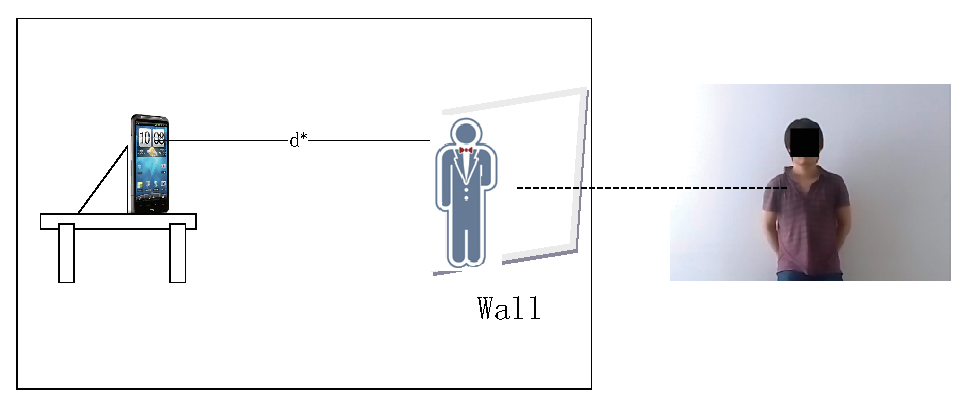
\includegraphics[width=3.5in]{epsfacedistance.eps}
\caption{Experimental setup for evaluation of distance estimation based on face detection}
\label{fig:distance-exp}
\end{figure}


Fig.~\ref{fig:distance-results} shows that the estimated distance is close to the actual distance using different phones.  The accuracy of distance estimation achieves nearly 82\%.
The error is caused by deviation in mapping image pixel count to actual distance.  We also observe that different phones have similar degree of accuracy.
By assuming the real face height  as 22cm (i.e., 8.734 inches), we use Eq.(2) to calculate the distance between camera and the face, which is 2.938m, very close to the actual distance of 2.4m.  We also calculate the area size to be 3.407$m^2$ while the actual size is 2.318$m^2$. This area estimation error is acceptable for detecting visual eavesdroppers.
%Fig.~\ref{fig:area-results} shows that the estimated area size is close to the actual area size using different phones.


\begin{figure}[H]\label{exp:expdistancechart}
\centering
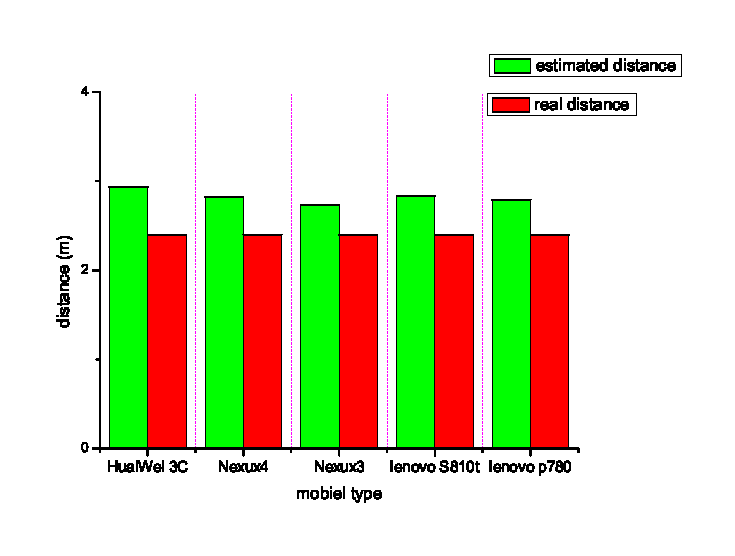
\includegraphics[width=2.7in]{epsdistancechart1.eps}
\caption{Estimated and actual distance of different phones}
\label{fig:distance-results}
\end{figure}

\begin{comment}
\begin{figure}[H]
\centering
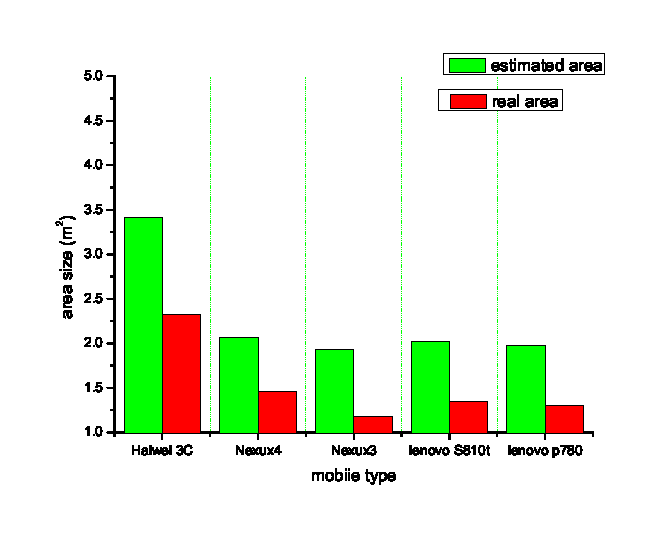
\includegraphics[width=2in]{epsdistancechart2.eps}
\caption{Estimated and actual monitoring area size of different phones}
\label{fig:area-results}
\end{figure}
\end{comment}

\subsection{Experiments on Face and Motion Detection} % Inside Camera View}
We use  publicly available face datasets such as BioID\cite{BioID}, Caltech\cite{jesorsky2001robust}, and FDDB\cite{jain2010fddb} datasets to evaluate the performance of our face detection, use the motion detection or tracking dataset such as PETS\cite{website:PETS} and part of the Yhyang tracking datasets to evaluate the performance of motion detection.

Our face detection achieves an accuracy of $81.7\%$, $95.3\%$ and $98.5\%$  using the FDDB, Caltech, and  BioID datasets respectively. Fig.~\ref{fig:face-results} is a sample of the face detection results. We observe the decrease of face detection accuracy with the lower clarity of the face in the image either due to presence of multiple faces in the images or low resolution of the image. We also notice that the face detection method always fails while the face does not directly face the camera.
\begin{figure}[H]
\centering
\includegraphics[width=3in]{epsfaces.eps}
\caption{Face detection results using publicly available datasets}
\label{fig:face-results}
\end{figure}

 The motion detection method achieves a high accuracy of more than $90\%$ using the classical datasets PETS2001. Fig.~\ref{fig:motion-results} is a sample result of motion detection. However, the method detects any moving object, not limited to moving person.  Since we are only interested in human, we combine  face detection  and motion detection.
 \begin{figure}[H]
\centering
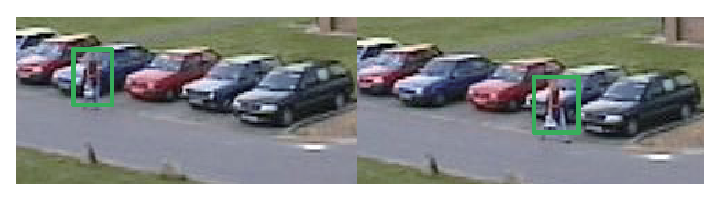
\includegraphics[width=3.5in]{epsmotionret.eps}
\caption{The experiments on motion detection in the PETS2001 datasets. }
\label{fig:motion-results}
\end{figure}


To evaluate the efficiency of our face detection which first removes the user-blocked area, we compare it against the method without blocked area removal  using images in the Caltech face datasets. The resolution of each image is $800\times600$, which is high enough to test the speed of face detection.  Fig.~\ref{fig:blocked-results} shows that our face detection method saves almost 20\% of the computation.
 \begin{figure}[H]
\centering
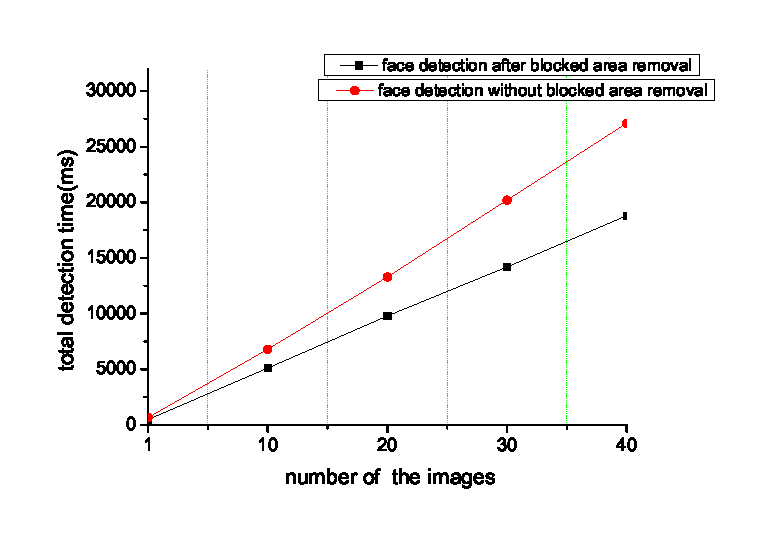
\includegraphics[width=3in]{epsfaceremoval.eps}
\caption{Face detection time}
\label{fig:blocked-results}
\end{figure}


\subsection{Experiments on Prediction of Visual Eavesdropper Location }


For predicting the location of a visual eavesdropper,  motion speed and direction is important to estimate the probability of the existing visual eavesdropping. In most situations,  motion direction takes a simple form, i.e., moving either left or right. Compared with  motion direction,  motion speed is more important in predicting the location of the visual eavesdropping. Therefore, we conduct the experiments on estimating motion speed to evaluate the accuracy of our method.

As Fig.~\ref{fig:speed-exp} shows, we let a person stand by the wall and go from  left  to  right. We record the time from the motion start to the motion end for several times. The width of the wall is 6.5 m and the speed can be calculated by dividing the length by the time. The average time is 7.5 seconds and the speed is 0.86 m/s. For our motion speed estimation, we use face detection method to locate the initial human position and consider the area that is three times of the face size,  below the face is the human body. We then use motion detection to track the human that includes the human face and body for getting the trajectories.

\begin{figure}[H]
\centering
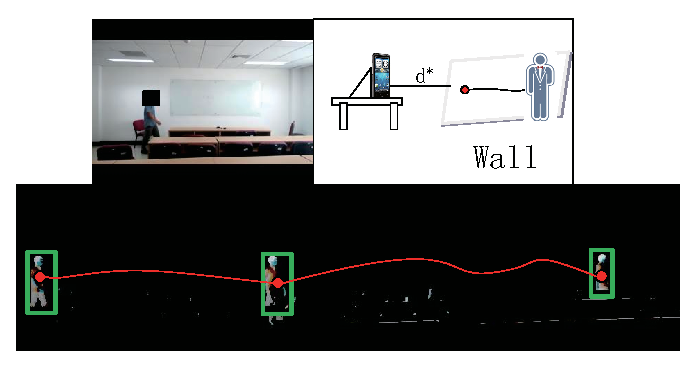
\includegraphics[width=3.5in]{epsmotion.eps}
\caption{Experimentsal setup for evaluating motion speed estimation. }
\label{fig:speed-exp}
\end{figure}
Considering that the distance $d^*$ is important for estimating the motion speed, we estimate the motion speed with known distance $d^*$ and also estimate motion speed in a designated area using time.
Fig.~\ref{fig:speed-results1} shows the estimated motion speed is close to the actual speed and achieves nearly $91.3\%$.




\begin{comment}
\subfigure{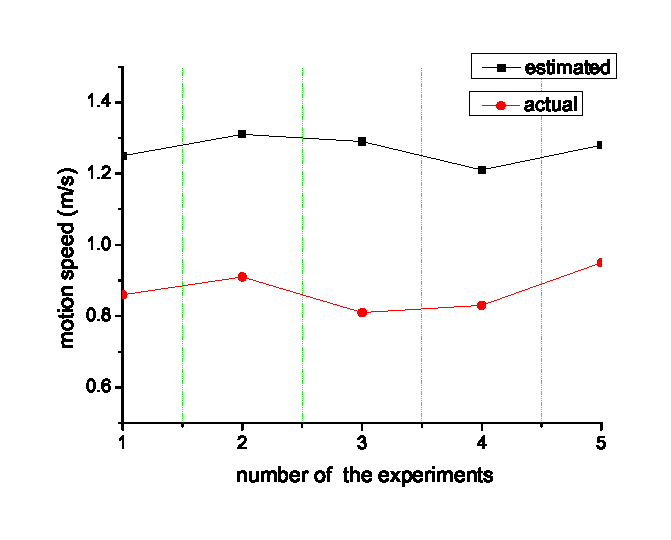
\includegraphics[width=3in]{epsmotionchart2.eps}}
\caption{Estimation of motion speed with estimated distance}
\label{fig:speed-results2}
\end{comment}


\subsection{Experiments on Overall Visual Eavesdropper Detection}
All the experiments discussed previously demonstrate that each component of our proposed visual eavesdropper detection method (i.e., area estimation, visible human detection,  and location prediction)  performs well using public datasets.  To validate that our overall approach works well in practice, we conducted the following experiments. We ask one person to use his phone as usual and another person tries to read his phone screen from behind while walking slowly behind him from left to right.
we set the angle of the camera view $\alpha_h$, $\alpha_v$ to $ 30^\circ $, $ 22^\circ $ and set the angle of potential eavesdropping $\beta$ to $ 60^\circ $. In this experiment, the time threshold \textit{t}(s) and $\tau(s)$  %learned by sensitivity of the environment perception
are set to be $12s$ and $8s$ respectively.  Fig.~\ref{fig:all-results} shows the results of these experiments.
The black area is the area blocked by phone user's face. The left figure shows  that the person behind the user is detected by face detection where the small rectangle is the detected human face; the right figure shows that the person is tracked by motion detection although the face is not detected where the large rectangle is the tracked human body. When the person moves out of the monitoring area, we get the probability to visual eavesdropping. When the time of the detected face is more than  threshold $\tau(s)$ or the time of the detected body is more than  threshold \textit{t}(s), the person behind is considered as a visual eavesdropper. The result of this experiment validates the effectiveness of our proposed visual eavesdropper detection.
\begin{figure}[H]
\centering
\includegraphics[width=3.5in]{expvee.eps}
\caption{Experiments on visual eavesdropper detection }
\label{fig:all-results}
\end{figure}


%{\bf Performance Summary. } Our finding include: (1) The area size calculated by the area estimation method is close to the real area size. (2) The estimation of the motion detection result can get approximate the motion speed and direction.(3) Proposed Human detection method has a robust detection result in the datasets.






\section{Conclusion}
In this paper, we define the problem of  visual  eavesdropping  and propose a method to detect it for preserving user privacy on smartphone. We conduct a variety of  experiments to evaluate the effectiveness of the proposed method  public datasets and real-world experiments.  This work can help alert people of potential eavesdropping.  In the future, we will complement this work by protecting user privacy via image distortion and masking when potential privacy leakage is detected.

Since MicroPrivacy is a CV based approach, its performance is limited by the performance of CV techniques.  When there are multiple people walking around the phone user or the background has significant light variation, the accuracy of face detection drops. Nevertheless, MicroPrivacy can work well in many scenarios, especially in a spacious place or  room with few people.  Our work shows that CV based methods have a great potential especially in the future when CV techniques become more robust and efficient. Further, there is a special scenario that a person may be looking in the direction of the smart-phone, he may not be looking at the smartphone. In this case,  MicroPrivacy takes a conservative approach by alerting the phone user anyway, without trying to differentiate between the two cases.  High energy consumption is another problem in CV based approaches on smartphones. To address this problem, a few pieces of work have already started investigating how to reduce the computation\cite{mobilevision}.  We believe these efforts along with the advances in smartphone hardware will make it acceptable to have CV based apps on smartphones. 

\bibliographystyle{IEEEtran}
\bibliography{IEEEabrv,mobile}




% that's all folks
\end{document}


